\documentclass{standalone}
\usepackage{tikz}
\usetikzlibrary{patterns, positioning}


\begin{document}
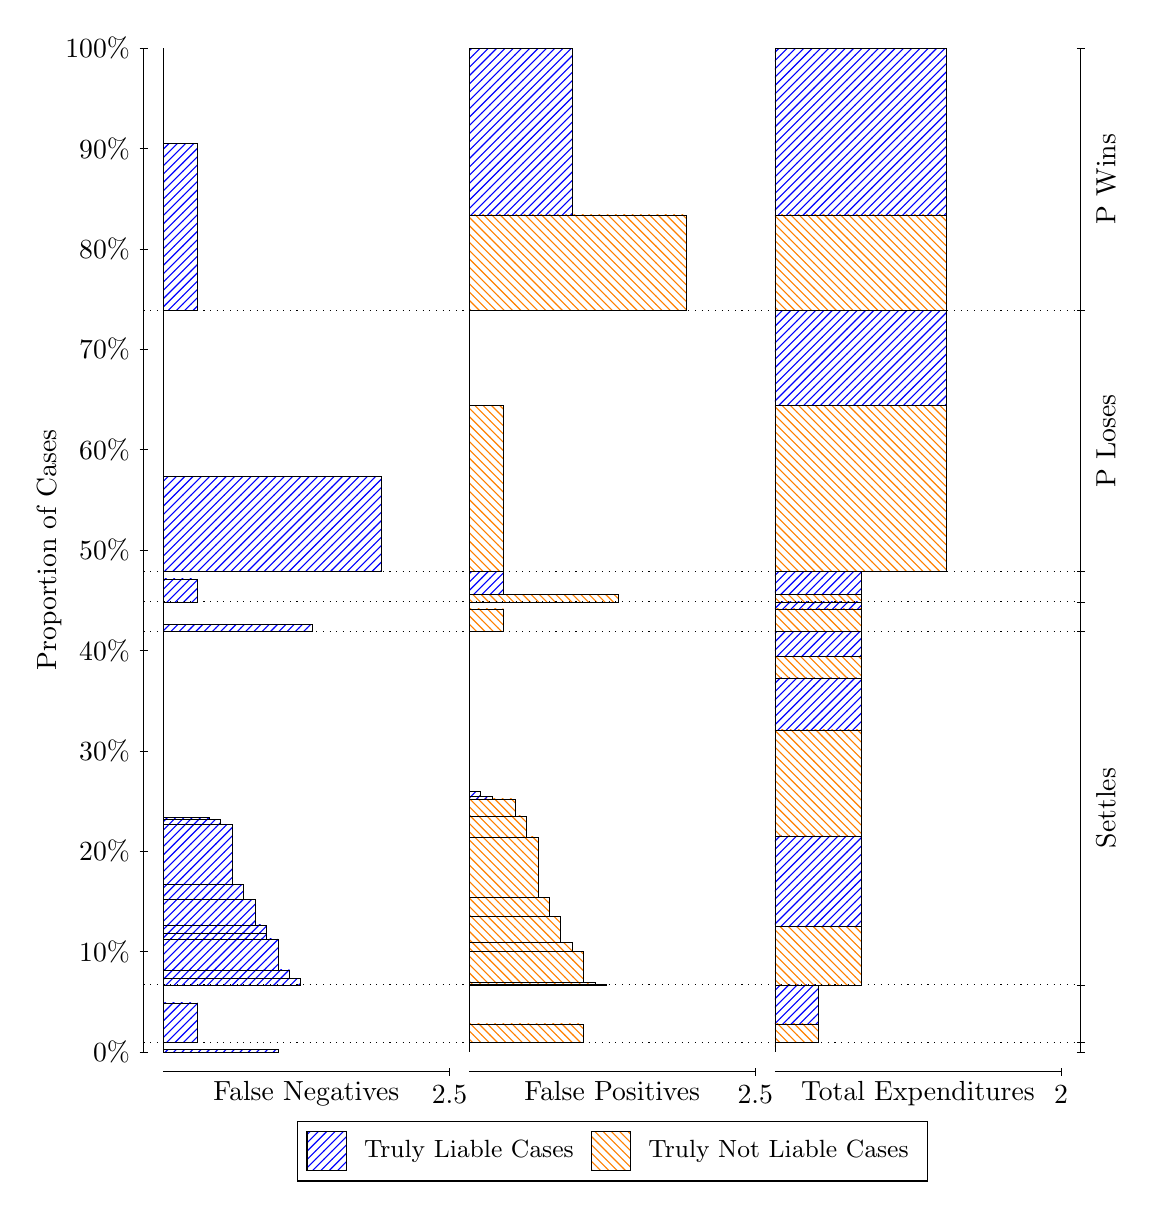
\begin{tikzpicture}
\draw[black, very thin] (1.5,1.75) -- (1.5,14.5);
\node[rotate=90, text=black, anchor=center] at (0.3, 8.125) {Proportion of Cases};
\draw[black, very thin] (1.45,1.75) -- (1.55,1.75);
\node[text=black, anchor=east] at (1.45, 1.75) {0\%};
\draw[black, very thin] (1.45,3.025) -- (1.55,3.025);
\node[text=black, anchor=east] at (1.45, 3.025) {10\%};
\draw[black, very thin] (1.45,4.3) -- (1.55,4.3);
\node[text=black, anchor=east] at (1.45, 4.3) {20\%};
\draw[black, very thin] (1.45,5.575) -- (1.55,5.575);
\node[text=black, anchor=east] at (1.45, 5.575) {30\%};
\draw[black, very thin] (1.45,6.85) -- (1.55,6.85);
\node[text=black, anchor=east] at (1.45, 6.85) {40\%};
\draw[black, very thin] (1.45,8.125) -- (1.55,8.125);
\node[text=black, anchor=east] at (1.45, 8.125) {50\%};
\draw[black, very thin] (1.45,9.4) -- (1.55,9.4);
\node[text=black, anchor=east] at (1.45, 9.4) {60\%};
\draw[black, very thin] (1.45,10.675) -- (1.55,10.675);
\node[text=black, anchor=east] at (1.45, 10.675) {70\%};
\draw[black, very thin] (1.45,11.95) -- (1.55,11.95);
\node[text=black, anchor=east] at (1.45, 11.95) {80\%};
\draw[black, very thin] (1.45,13.225) -- (1.55,13.225);
\node[text=black, anchor=east] at (1.45, 13.225) {90\%};
\draw[black, very thin] (1.45,14.5) -- (1.55,14.5);
\node[text=black, anchor=east] at (1.45, 14.5) {100\%};

\draw[black, very thin] (13.4,1.75) -- (13.4,14.5);
\draw[black, very thin] (13.35,1.75) -- (13.45,1.75);
\node[anchor=west] at (13.35, 1.75) {};
\draw[black, very thin] (13.35,1.8756) -- (13.45,1.8756);
\node[anchor=west] at (13.35, 1.8756) {};
\draw[black, very thin] (13.35,2.6025) -- (13.45,2.6025);
\node[anchor=west] at (13.35, 2.6025) {};
\draw[black, very thin] (13.35,7.0952) -- (13.45,7.0952);
\node[anchor=west] at (13.35, 7.0952) {};
\draw[black, very thin] (13.35,7.4673) -- (13.45,7.4673);
\node[anchor=west] at (13.35, 7.4673) {};
\draw[black, very thin] (13.35,7.8499) -- (13.45,7.8499);
\node[anchor=west] at (13.35, 7.8499) {};
\draw[black, very thin] (13.35,11.172) -- (13.45,11.172);
\node[anchor=west] at (13.35, 11.172) {};
\draw[black, very thin] (13.35,14.5) -- (13.45,14.5);
\node[anchor=west] at (13.35, 14.5) {};

\draw[black, very thin, pattern color=blue, pattern=north east lines] (1.75,1.75) rectangle (3.2033,1.7845);
\draw[black, very thin, pattern color=orange, pattern=north west lines] (1.75,1.7845) rectangle (1.75,1.8756);
\draw[black, very thin, pattern color=blue, pattern=north east lines] (1.75,1.8756) rectangle (2.186,2.3723);
\draw[black, very thin, pattern color=orange, pattern=north west lines] (1.75,2.3723) rectangle (1.75,2.6025);
\draw[black, very thin, pattern color=blue, pattern=north east lines] (1.75,2.6025) rectangle (3.494,2.682);
\draw[black, very thin, pattern color=blue, pattern=north east lines] (1.75,2.682) rectangle (3.3487,2.7927);
\draw[black, very thin, pattern color=blue, pattern=north east lines] (1.75,2.7927) rectangle (3.2033,3.1864);
\draw[black, very thin, pattern color=blue, pattern=north east lines] (1.75,3.1864) rectangle (3.058,3.2626);
\draw[black, very thin, pattern color=blue, pattern=north east lines] (1.75,3.2626) rectangle (3.058,3.3631);
\draw[black, very thin, pattern color=blue, pattern=north east lines] (1.75,3.3631) rectangle (2.9127,3.6928);
\draw[black, very thin, pattern color=blue, pattern=north east lines] (1.75,3.6928) rectangle (2.7673,3.8809);
\draw[black, very thin, pattern color=blue, pattern=north east lines] (1.75,3.8809) rectangle (2.622,4.6368);
\draw[black, very thin, pattern color=blue, pattern=north east lines] (1.75,4.6368) rectangle (2.4767,4.7017);
\draw[black, very thin, pattern color=blue, pattern=north east lines] (1.75,4.7017) rectangle (2.3313,4.7341);
\draw[black, very thin, pattern color=orange, pattern=north west lines] (1.75,4.7341) rectangle (1.75,7.0952);
\draw[black, very thin, pattern color=blue, pattern=north east lines] (1.75,7.0952) rectangle (3.6393,7.1849);
\draw[black, very thin, pattern color=orange, pattern=north west lines] (1.75,7.1849) rectangle (1.75,7.4673);
\draw[black, very thin, pattern color=blue, pattern=north east lines] (1.75,7.4673) rectangle (2.186,7.7594);
\draw[black, very thin, pattern color=orange, pattern=north west lines] (1.75,7.7594) rectangle (1.75,7.8499);
\draw[black, very thin, pattern color=blue, pattern=north east lines] (1.75,7.8499) rectangle (4.5113,9.0627);
\draw[black, very thin, pattern color=orange, pattern=north west lines] (1.75,9.0627) rectangle (1.75,11.172);
\draw[black, very thin, pattern color=blue, pattern=north east lines] (1.75,11.172) rectangle (2.186,13.29);
\draw[black, very thin, pattern color=orange, pattern=north west lines] (1.75,13.29) rectangle (1.75,14.5);
\draw[black, very thin, pattern color=orange, pattern=north west lines] (5.6333,1.75) rectangle (5.6333,1.8411);
\draw[black, very thin, pattern color=blue, pattern=north east lines] (5.6333,1.8411) rectangle (5.6333,1.8756);
\draw[black, very thin, pattern color=orange, pattern=north west lines] (5.6333,1.8756) rectangle (7.0867,2.1058);
\draw[black, very thin, pattern color=blue, pattern=north east lines] (5.6333,2.1058) rectangle (5.6333,2.6025);
\draw[black, very thin, pattern color=orange, pattern=north west lines] (5.6333,2.6025) rectangle (7.3773,2.6107);
\draw[black, very thin, pattern color=orange, pattern=north west lines] (5.6333,2.6107) rectangle (7.232,2.6317);
\draw[black, very thin, pattern color=orange, pattern=north west lines] (5.6333,2.6317) rectangle (7.0867,3.0242);
\draw[black, very thin, pattern color=orange, pattern=north west lines] (5.6333,3.0242) rectangle (6.9413,3.1431);
\draw[black, very thin, pattern color=orange, pattern=north west lines] (5.6333,3.1431) rectangle (6.796,3.4708);
\draw[black, very thin, pattern color=orange, pattern=north west lines] (5.6333,3.4708) rectangle (6.6507,3.7139);
\draw[black, very thin, pattern color=orange, pattern=north west lines] (5.6333,3.7139) rectangle (6.5053,4.4802);
\draw[black, very thin, pattern color=orange, pattern=north west lines] (5.6333,4.4802) rectangle (6.36,4.7484);
\draw[black, very thin, pattern color=orange, pattern=north west lines] (5.6333,4.7484) rectangle (6.2147,4.9635);
\draw[black, very thin, pattern color=blue, pattern=north east lines] (5.6333,4.9635) rectangle (5.924,4.9959);
\draw[black, very thin, pattern color=blue, pattern=north east lines] (5.6333,4.9959) rectangle (5.7787,5.0608);
\draw[black, very thin, pattern color=blue, pattern=north east lines] (5.6333,5.0608) rectangle (5.6333,7.0952);
\draw[black, very thin, pattern color=orange, pattern=north west lines] (5.6333,7.0952) rectangle (6.0693,7.3776);
\draw[black, very thin, pattern color=blue, pattern=north east lines] (5.6333,7.3776) rectangle (5.6333,7.4673);
\draw[black, very thin, pattern color=orange, pattern=north west lines] (5.6333,7.4673) rectangle (7.5227,7.5579);
\draw[black, very thin, pattern color=blue, pattern=north east lines] (5.6333,7.5579) rectangle (6.0693,7.8499);
\draw[black, very thin, pattern color=orange, pattern=north west lines] (5.6333,7.8499) rectangle (6.0693,9.9595);
\draw[black, very thin, pattern color=blue, pattern=north east lines] (5.6333,9.9595) rectangle (5.6333,11.172);
\draw[black, very thin, pattern color=orange, pattern=north west lines] (5.6333,11.172) rectangle (8.3947,12.382);
\draw[black, very thin, pattern color=blue, pattern=north east lines] (5.6333,12.382) rectangle (6.9413,14.5);
\draw[black, very thin, pattern color=orange, pattern=north west lines] (9.5167,1.75) rectangle (9.5167,1.8411);
\draw[black, very thin, pattern color=blue, pattern=north east lines] (9.5167,1.8411) rectangle (9.5167,1.8756);
\draw[black, very thin, pattern color=orange, pattern=north west lines] (9.5167,1.8756) rectangle (10.062,2.1058);
\draw[black, very thin, pattern color=blue, pattern=north east lines] (9.5167,2.1058) rectangle (10.062,2.6025);
\draw[black, very thin, pattern color=orange, pattern=north west lines] (9.5167,2.6025) rectangle (10.607,3.3437);
\draw[black, very thin, pattern color=blue, pattern=north east lines] (9.5167,3.3437) rectangle (10.607,4.4942);
\draw[black, very thin, pattern color=orange, pattern=north west lines] (9.5167,4.4942) rectangle (10.607,5.8418);
\draw[black, very thin, pattern color=blue, pattern=north east lines] (9.5167,5.8418) rectangle (10.607,6.5019);
\draw[black, very thin, pattern color=orange, pattern=north west lines] (9.5167,6.5019) rectangle (10.607,6.7741);
\draw[black, very thin, pattern color=blue, pattern=north east lines] (9.5167,6.7741) rectangle (10.607,7.0952);
\draw[black, very thin, pattern color=orange, pattern=north west lines] (9.5167,7.0952) rectangle (10.607,7.3776);
\draw[black, very thin, pattern color=blue, pattern=north east lines] (9.5167,7.3776) rectangle (10.607,7.4673);
\draw[black, very thin, pattern color=orange, pattern=north west lines] (9.5167,7.4673) rectangle (10.607,7.5579);
\draw[black, very thin, pattern color=blue, pattern=north east lines] (9.5167,7.5579) rectangle (10.607,7.8499);
\draw[black, very thin, pattern color=orange, pattern=north west lines] (9.5167,7.8499) rectangle (11.697,9.9595);
\draw[black, very thin, pattern color=blue, pattern=north east lines] (9.5167,9.9595) rectangle (11.697,11.172);
\draw[black, very thin, pattern color=orange, pattern=north west lines] (9.5167,11.172) rectangle (11.697,12.382);
\draw[black, very thin, pattern color=blue, pattern=north east lines] (9.5167,12.382) rectangle (11.697,14.5);
\draw[black, dotted] (1.5,1.8756) -- (13.4,1.8756);
\draw[black, dotted] (1.5,2.6025) -- (13.4,2.6025);
\draw[black, dotted] (1.5,7.0952) -- (13.4,7.0952);
\draw[black, dotted] (1.5,7.4673) -- (13.4,7.4673);
\draw[black, dotted] (1.5,7.8499) -- (13.4,7.8499);
\draw[black, dotted] (1.5,11.172) -- (13.4,11.172);
\draw[black, very thin] (1.75,1.5) -- (5.3833,1.5);
\node[text=black, anchor=north] at (3.5667, 1.5) {False Negatives};
\draw[black, very thin] (5.3833,1.45) -- (5.3833,1.55);
\node[text=black, anchor=north] at (5.3833, 1.45) {2.5};

\draw[black, very thin] (5.6333,1.5) -- (9.2667,1.5);
\node[text=black, anchor=north] at (7.45, 1.5) {False Positives};
\draw[black, very thin] (9.2667,1.45) -- (9.2667,1.55);
\node[text=black, anchor=north] at (9.2667, 1.45) {2.5};

\draw[black, very thin] (9.5167,1.5) -- (13.15,1.5);
\node[text=black, anchor=north] at (11.333, 1.5) {Total Expenditures};
\draw[black, very thin] (13.15,1.45) -- (13.15,1.55);
\node[text=black, anchor=north] at (13.15, 1.45) {2};



\node[text=black, centered, rotate=90] at (13.72, 4.8488) {Settles};


\node[text=black, centered, rotate=90] at (13.72, 9.5111) {P Loses};
\node[text=black, centered, rotate=90] at (13.72, 12.836) {P Wins};

\draw (7.449999999999999,1.5) node[draw=none] (baseCoordinate) {};
\begin{scope}[align=center]
        \matrix[scale=0.5, draw=black, below=0.5cm of baseCoordinate, nodes={draw}, column sep=0.1cm]{
            \node[rectangle, draw, minimum width=0.5cm, minimum height=0.5cm, pattern color=blue, pattern=north east lines] {}; &
            \node[draw=none, font=\small, text=black] (B) {Truly Liable Cases}; &
            \node[rectangle, draw, minimum width=0.5cm, minimum height=0.5cm, pattern color=orange, pattern=north west lines] {}; &
            \node[draw=none, font=\small, text=black] (B) {Truly Not Liable Cases}; \\
            };
\end{scope}

\end{tikzpicture}
\end{document}